\documentclass{article}
\usepackage[left=0.5in,top=0.5in,right=0.5in,bottom=0.5in]{geometry}
\usepackage[english]{babel}
\usepackage[utf8]{inputenc}
\usepackage[table]{xcolor}
\usepackage{amssymb,amsmath,amsthm}
\usepackage{changepage,threeparttable}
\usepackage{booktabs,multirow}
\usepackage{graphicx}
\usepackage{soul}
\def\R#1#2{\(#1_{\text{\tiny#2}}\)}
\def\C{\(\mu F\)}
\def\OHM{\(k\Omega \)}
\graphicspath{{./images/}}
\title{Lab 6: The Impedance of Capacitors}
\author{Philip Kim}
\date{\today}
\begin{document}
\maketitle
\vspace*{-1cm}
\begin{table}[!htp]\centering
  \subsection*{Part 1}
  \begin{tabular}{|c|c|c|c|c|c|c|c|c|c|c|}\hline
  \multicolumn{11}{|c|}{\textbf{Table 1: Impedance of a Capacitor}} \\\hline
  C & R & \R{V}{RC} & \R{V}{R} & V/DIV for \R{V}{R} & \R{f}{gen} & \R{f}{osc} & \R{I}{R} & \R{V}{C} & \R{X}{C,exp} & \R{X}{C,the} \\\hline
  0.10\C & 1\OHM\ & 2.67V & 0.81V & 2V & 523Hz & 539Hz & 0.00081 & 2.5442V & 3140.9 & 2952.8 \\\hline
  0.22\C & 1\OHM\ & 2.67V & 1.54V & 2V & 523Hz & 539Hz & 0.0015 & 2.1811V & 1454.1 & 1342.2 \\\hline
  0.33\C & 1\OHM\ & 2.67V & 2.02V & 2V & 523Hz & 539Hz & 0.0020 & 1.7460V & 873.0 & 894.8 \\\hline
  0.47\C & 1\OHM\ & 2.67V & 2.27V & 2V & 523Hz & 539Hz & 0.0023 & 1.4057V & 611.2 & 628.3 \\\hline
  0.68\C & 1\OHM\ & 2.67V & 2.43V & 2V & 523Hz & 539Hz & 0.0024 & 1.1063V & 460.9 & 434.2 \\\hline
  1.00\C & 1\OHM\ & 2.67V & 2.51V & 2V & 523Hz & 539Hz & 0.0025 & 0.9104V & 364.2 & 295.3 \\\hline
  \end{tabular}
\end{table}
\begin{center}
  \subsection*{\R{R}{RC}}
  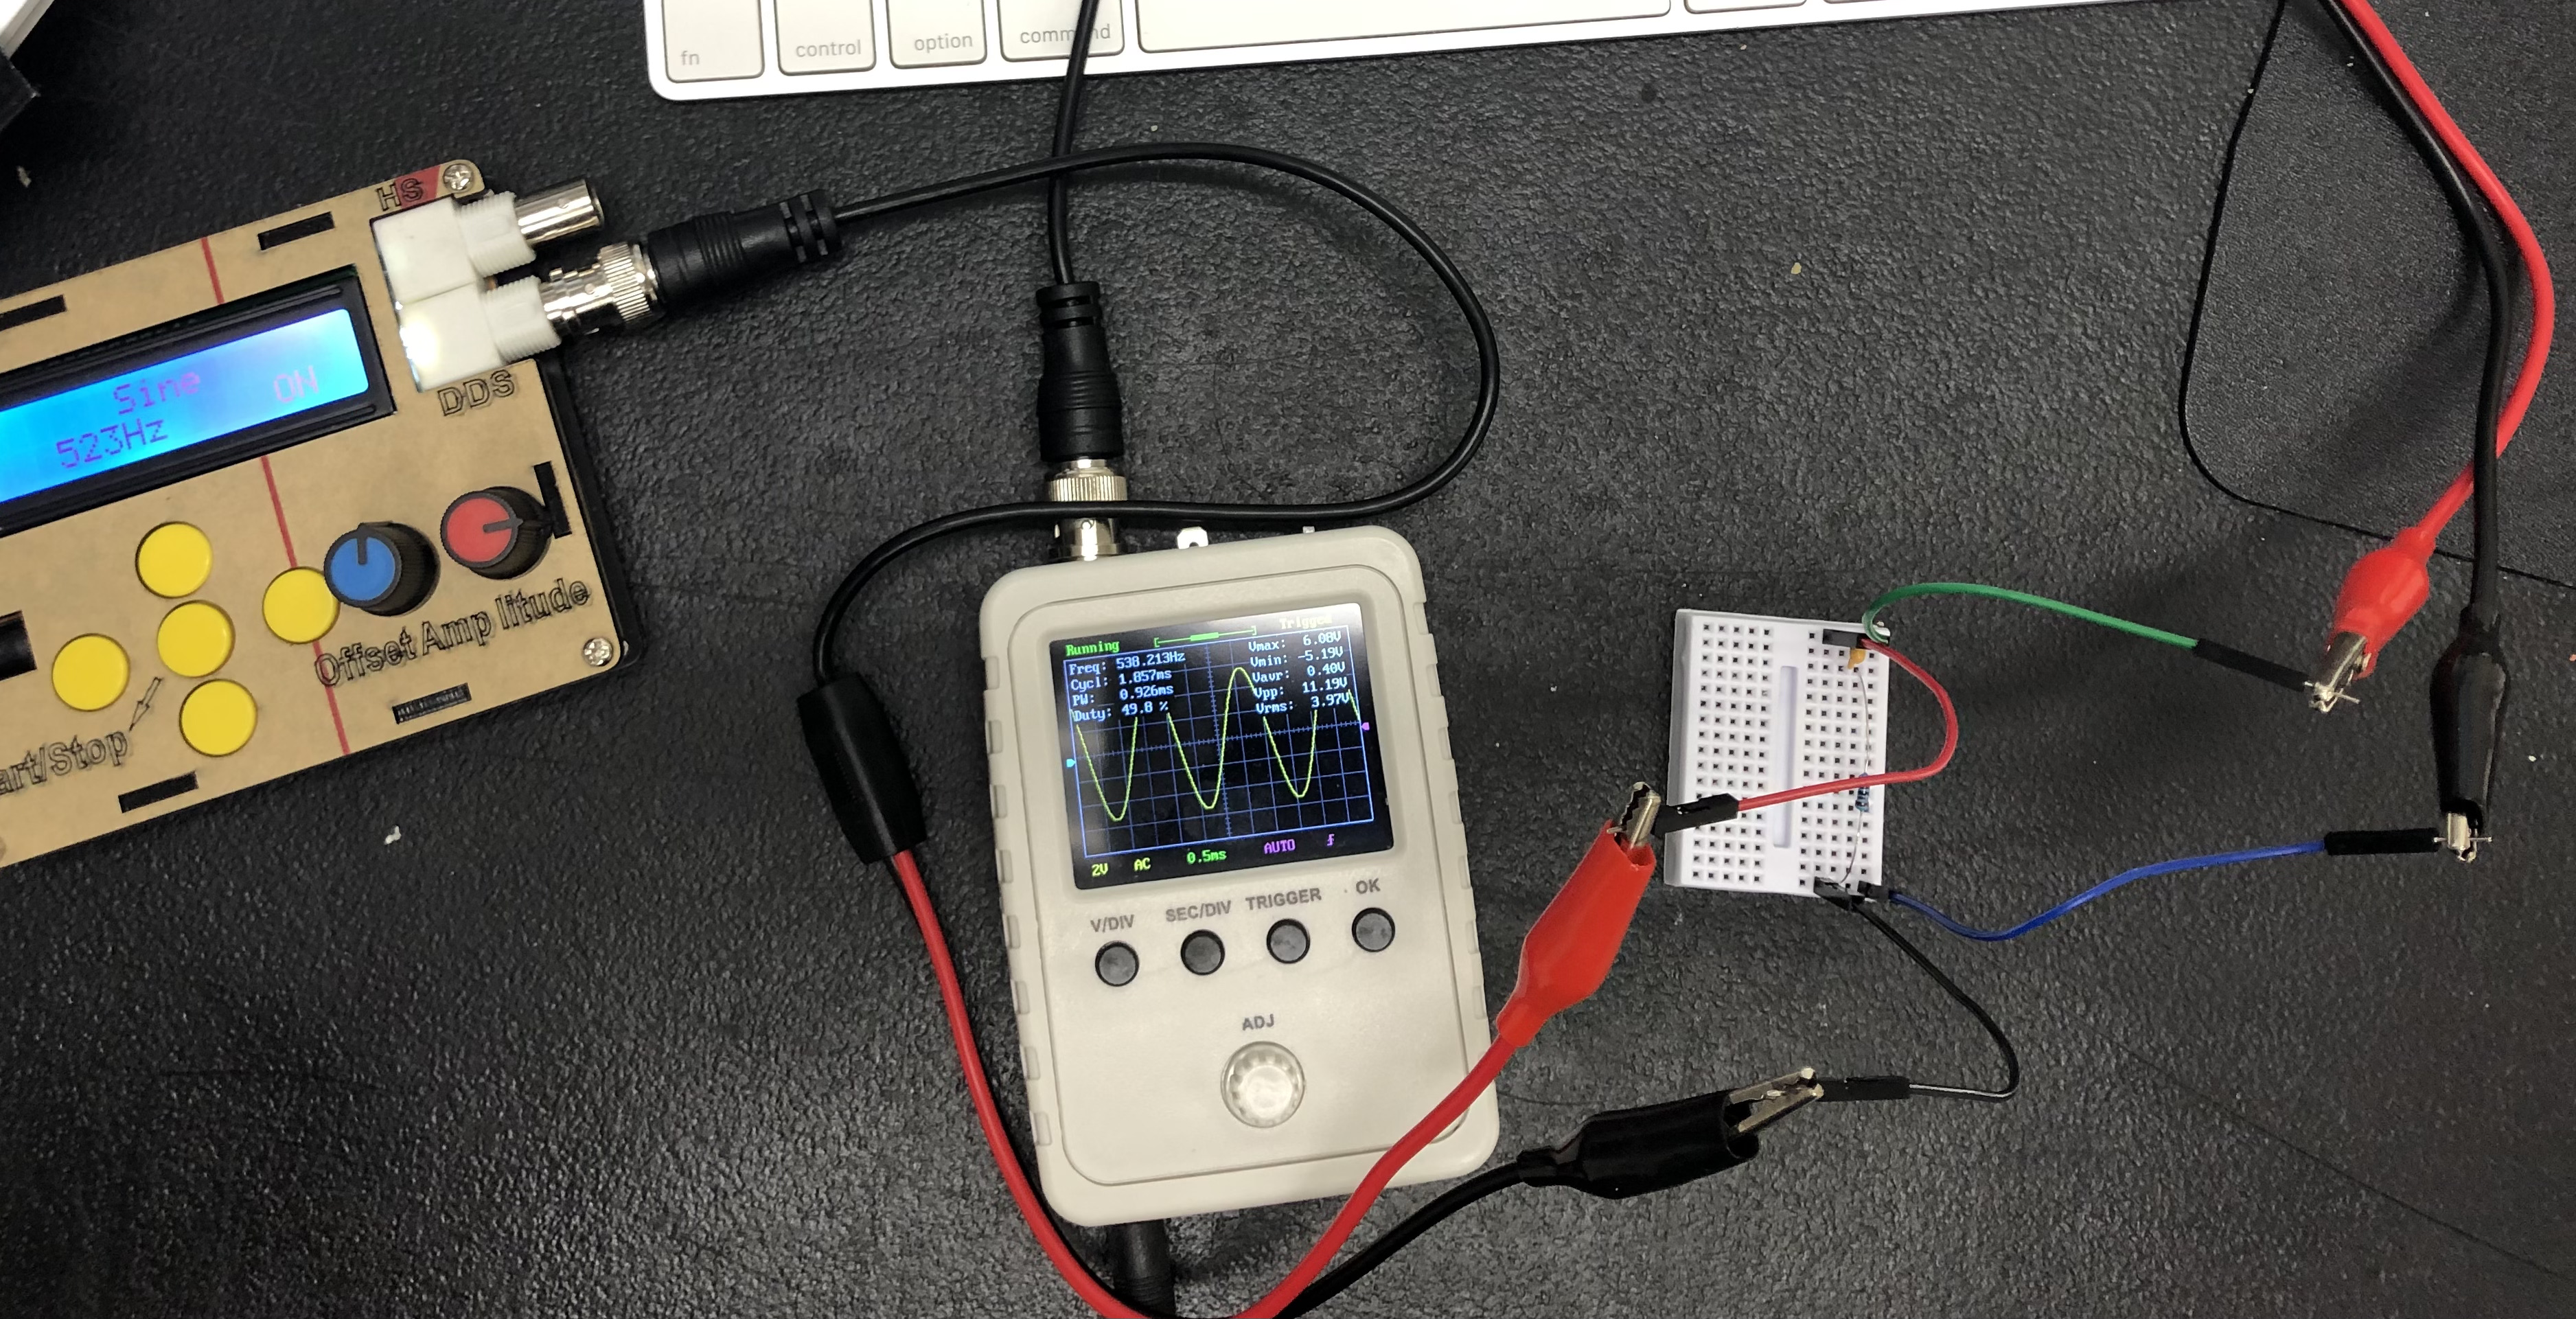
\includegraphics[scale=0.1]{Vrc.jpeg}
  \subsection*{\R{R}{C}}
  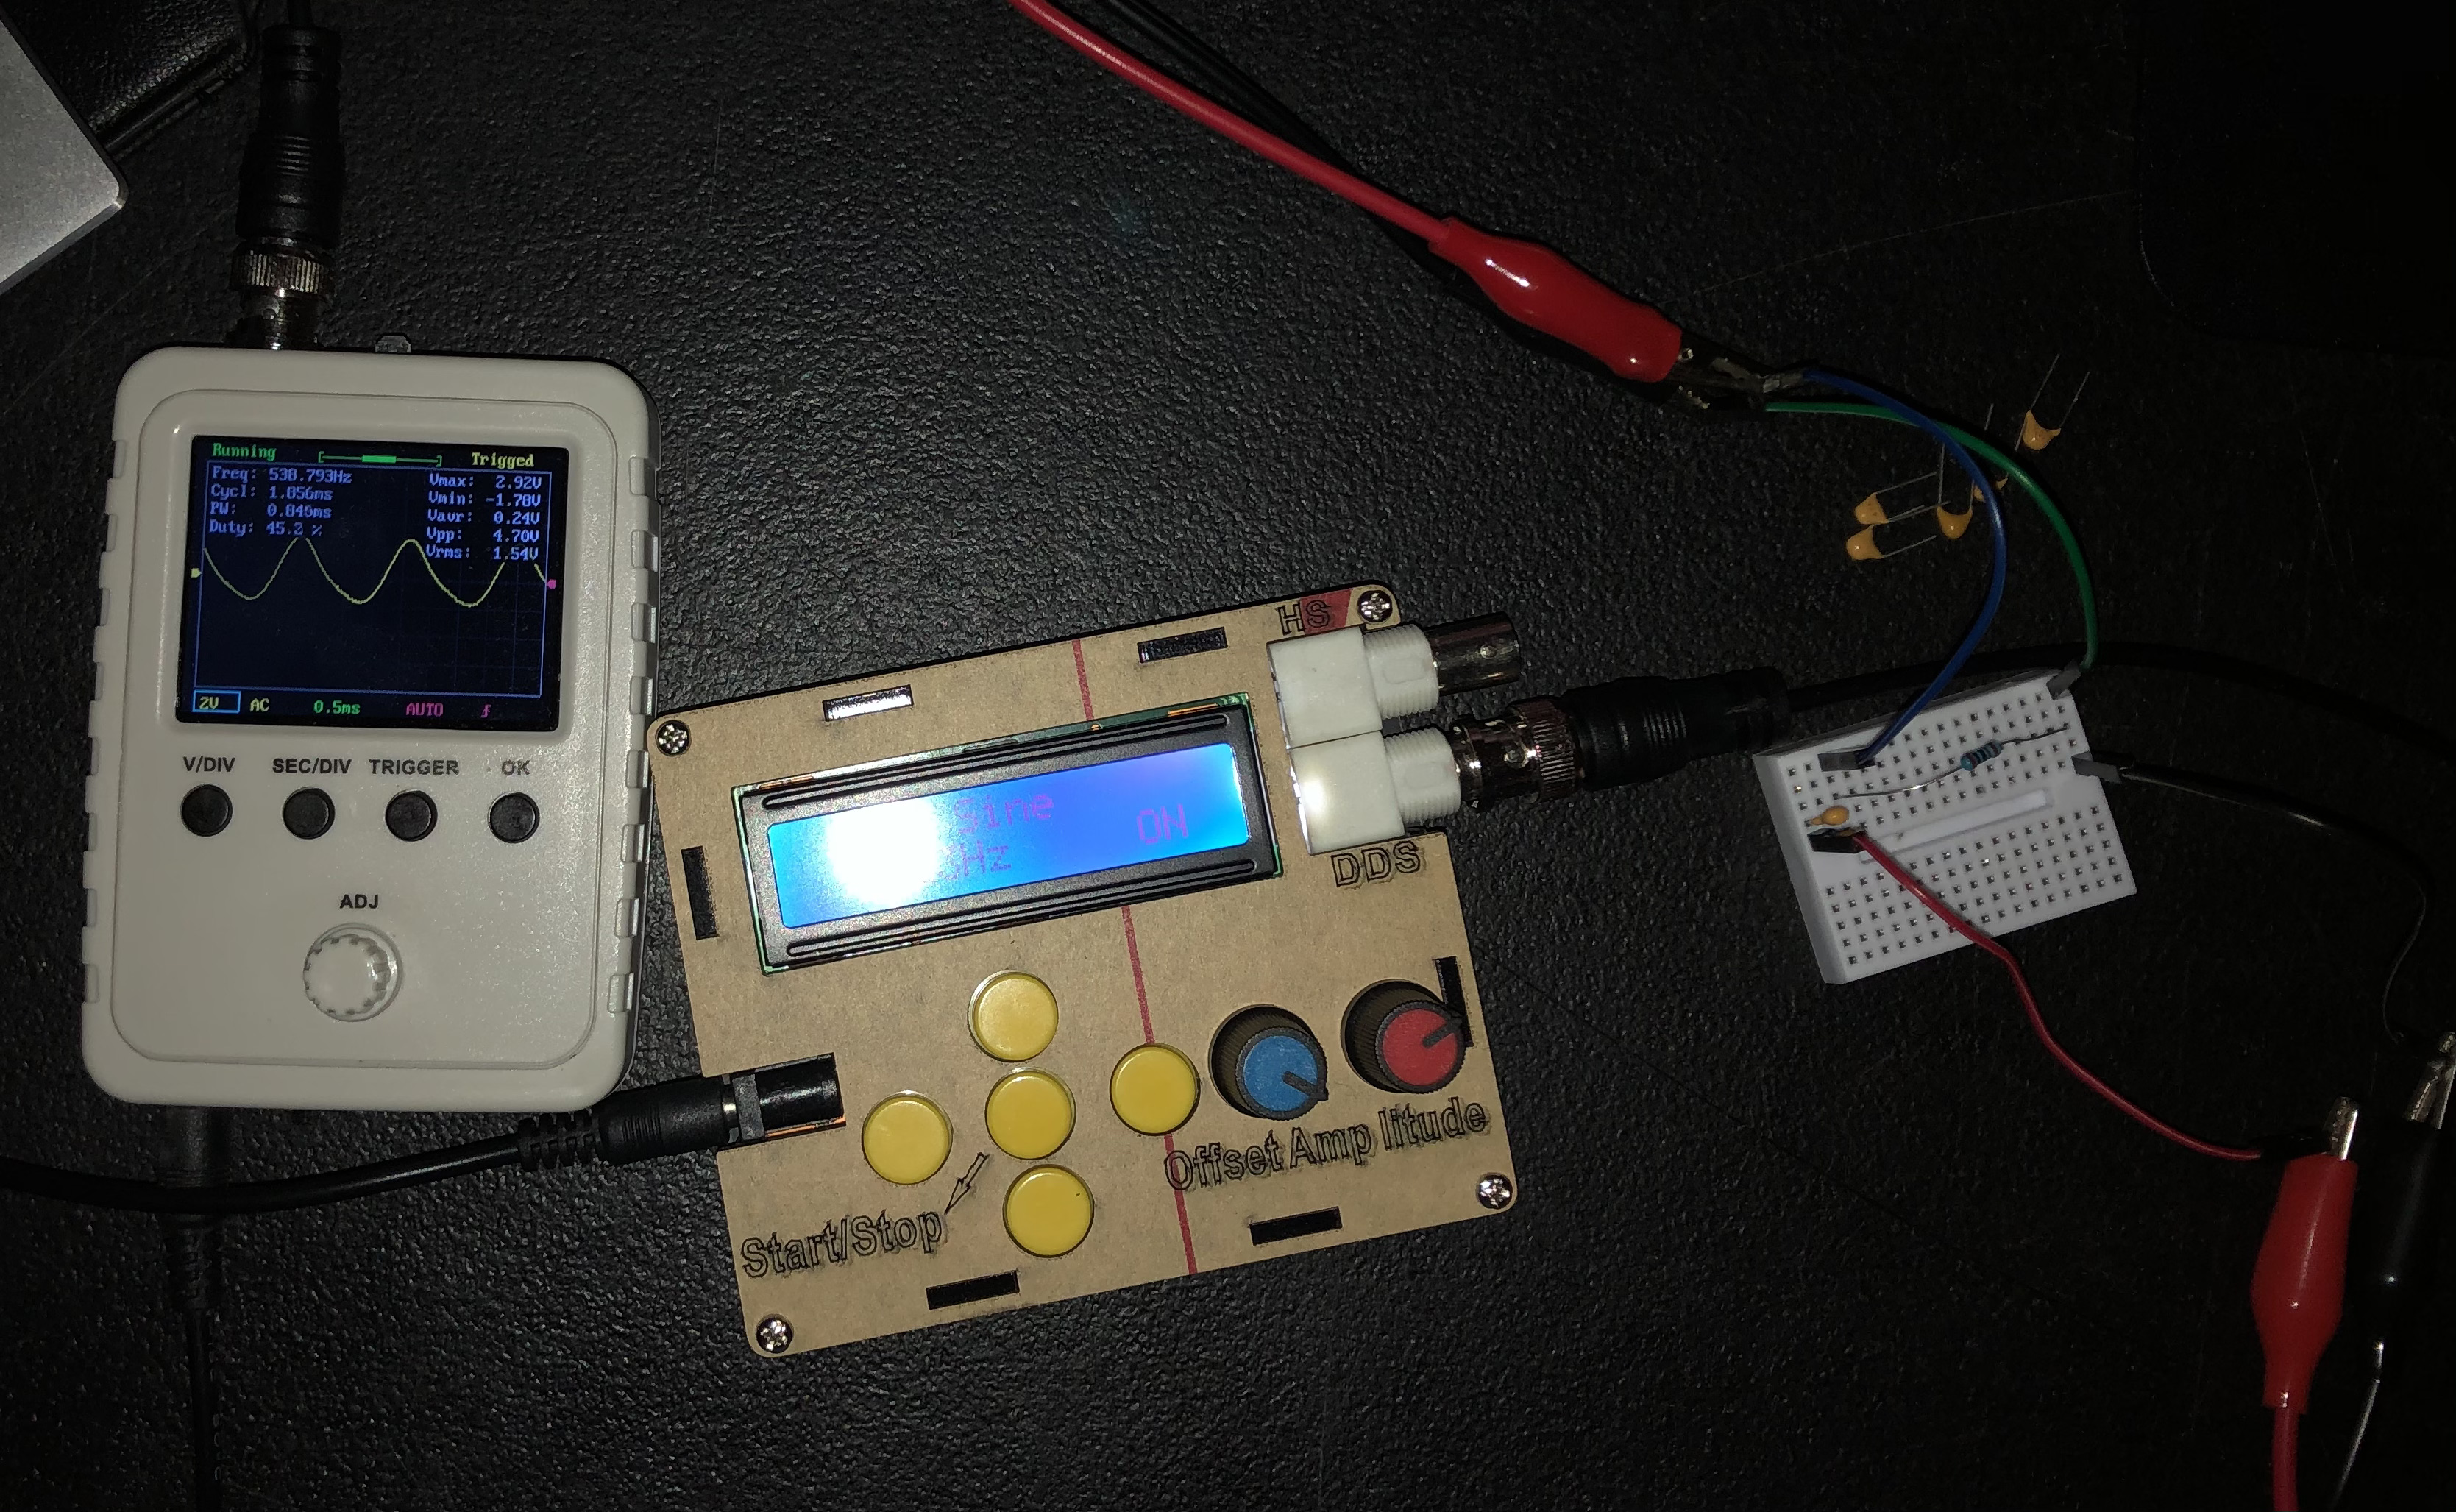
\includegraphics[scale=0.1]{Vr.jpeg}
\end{center}
\begin{center}
  \subsection*{Graph 1}
  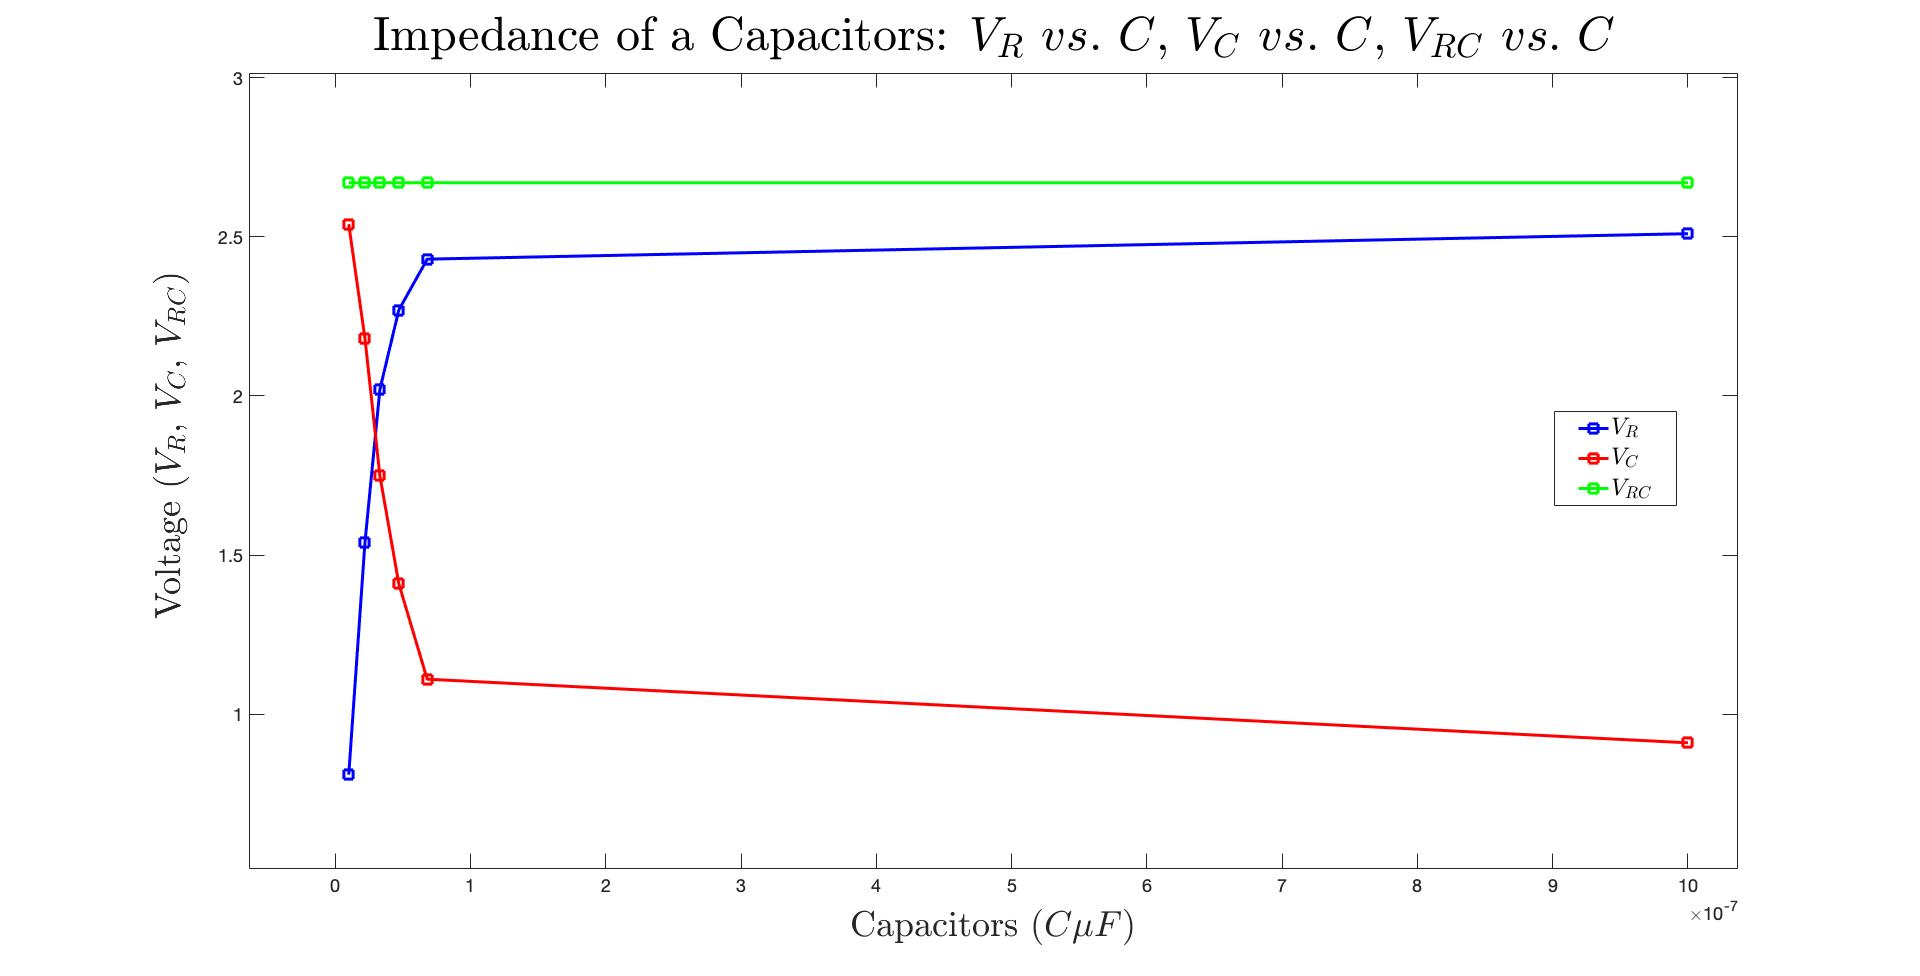
\includegraphics[scale=0.25]{graph1.jpg}
  \subsection*{Graph 2}
  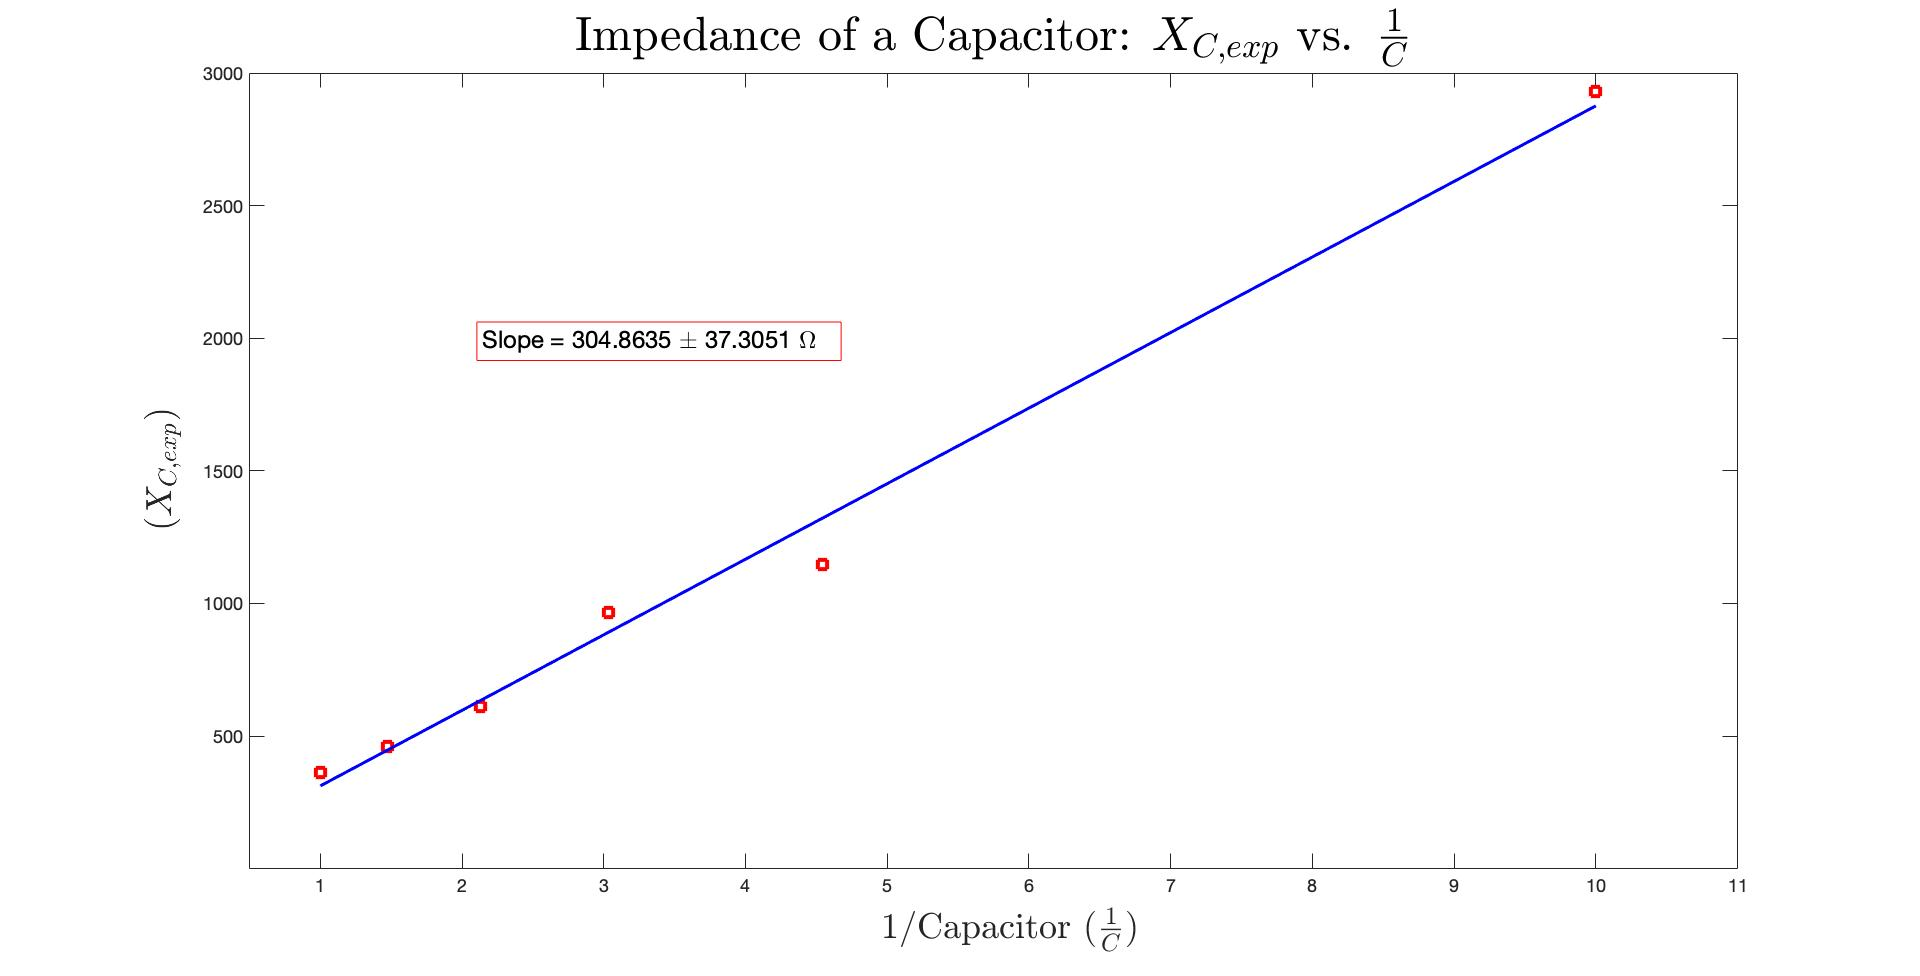
\includegraphics[scale=0.25]{graph2.jpg}
\end{center}
\begin{center}
\subsection*{Discussion 1}
  \begin{enumerate}
    \item What slope do you find for graph 2 and how does it compare to your expectation?
    \begin{itemize}
      \item Experimental Slope = 314.5 \(\pm \) 28.1\(\Omega \)
      \item Theoretical Slope = 295.3 \(\pm \) 0.0164\(\Omega \)
    \end{itemize}
      \item What does a deviation from the linear fit indicate? How would you correct for the ones with the largest error?
    \begin{itemize}
      \item These deviation indicates that the capacitors are not accurate as mentioned in the manual. Replacing capacitors with better capacitors would be the obvious option, but in our case we can calculate the theoretical and adjust the amplitude to reach a closer approximation to the theoretical value or use different capacitors values.
    \end{itemize}
  \end{enumerate}
\end{center}
\end{document}
